\begin{definition}[Ordered Crossover]
    The \textit{ordered crossover} operator takes two parent chromosomes. Through a series of steps, it ensures that 
    the offspring chromosomes inherit the order of sequences or genes from both parents. Formally, the ordered 
    crossover is represented as:

    \begin{equation}
        X_\mathrm{ox}(P: \mathbb{P},\, \rho_\textbf{i}: [0,\, 1],\, \rho_\mathbf{c}: [0,\, 1],\, e: \{0,\, 1\}) 
            \to \mathbb{P}
    \end{equation}

    where:

    \begin{itemize}
    \item \(P\) denotes a population of ordered chromosomes.
    \item \(\rho_\textbf{i}\) is the probability of applying the crossover to an individual.
    \item \(\rho_\mathbf{c}\) represents the chance of employing the ordered crossover on a chromosome.
    \item \(e\) is a boolean value that determines whether the same individual can be used more than once as a parent.
    \end{itemize}
\end{definition}

There are multiple implementations of the ordered crossover operator. The 
following displays the variant used in the \textit{Keen} framework:

\begin{code}{
    OX algorithm as implemented in the \textit{Keen} framework. For simplicity, we represent chromosomes as arrays, 
    meaning that \texttt{output1[i] = input1[i]} signifies that the \texttt{i}-th gene in \texttt{output1} will be
    assigned the value of the \texttt{i}-th gene in \texttt{input1}. \texttt{input1} and \texttt{input2} are the parent 
    chromosomes, while \texttt{output1} and \texttt{output2} are the offspring chromosomes. All arrays are assumed to
    be of the same size.
}{
    label={lst:keen:op:cx:ox}
}{kotlin}
    val (index1, index2) = random.indices in input1
    val crossSection = input1[index1..index2]
    for (i in 0..input1.size) {
        if (i < index1 or i >= index2) {
            if (input2[i] not in crossSection) {
                output1[i] = input2[i]
            }
            if (input1[i] not in crossSection) {
                output2[i] = input1[i]
            }
        }
    }
    return output1, output2
\end{code}

In this approach, a random section from the first parent chromosome is copied 
to an offspring chromosome in the same position. Subsequently, genes from the 
second parent chromosome, not in the copied section, fill the offspring in 
the same order. The second offspring chromosome uses the second parent 
chromosome for the copied section and the first parent for the remaining 
genes. For a visual elucidation of this process, refer to 
\vref{fig:keen:op:cx:ox}.

\begin{figure}[ht!]
    \centering
    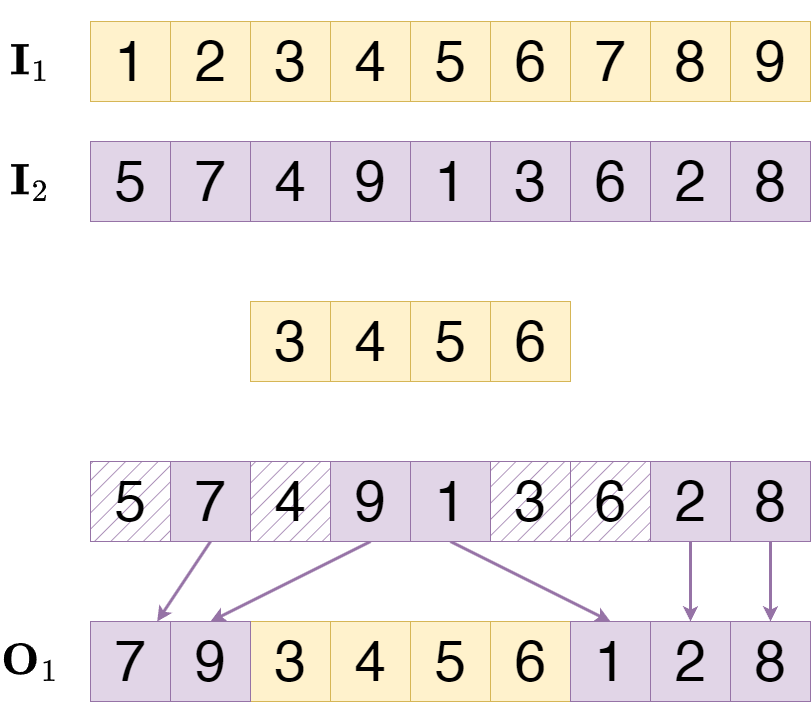
\includegraphics[width=0.33\textwidth]{img/keen/OX.png}
    \caption{Ordered Crossover (OX) operator.}
    \label{fig:keen:op:cx:ox}
\end{figure}
